\documentclass[a4paper]{article}
\usepackage[spanish]{babel}
\title{Trabajo Práctico 2}

\usepackage[utf8]{inputenc}
\usepackage{caratula}
\usepackage{graphicx}
\usepackage{color}
\usepackage{listings}
\usepackage{float}
\usepackage{amsmath}
\usepackage{amsfonts}
\usepackage{amssymb}


\setlength{\leftmargin}{2cm}
\setlength{\rightmargin}{2cm}
\setlength{\oddsidemargin}{-1cm}
\setlength{\evensidemargin}{-1cm}
\setlength{\topmargin}{-1cm}
\setlength{\textwidth}{18cm}
\setlength{\textheight}{25cm}

\usepackage{fancyhdr}
\pagestyle{fancy}
\fancyhf{}
\fancyhead [LO,LE]{\scriptsize Trabajo Práctico N$^{\circ}$2}
\fancyhead [RO,RE]{\scriptsize Mancuso, Mataloni, Tolchinsky}
\fancyfoot[CE,CO]{\thepage}
\renewcommand{\footrulewidth}{0.4pt}

\usepackage[pdftex, bookmarks=true, colorlinks, citecolor=black, linkcolor=black]{hyperref}
\usepackage{multirow}

\begin{document}

\materia{Métodos Numéricos}
\submateria{Primer Cuatrimestre de 2012}
\titulo{Filtrado de imágenes resueltas con ecuaciones lineales. }
\subtitulo{ Ecuaciones Lineales, Filtro de imagen }
\grupo{Trabajo Práctico N$^{\circ}$2}

\integrante{Mancuso, Emiliano}{597/07}{emiliano.mancuso@gmail.com}
\integrante{Mataloni, Alejandro}{706/07}{amataloni@gmail.com}
\integrante{Tolchinsky, Lucas}{591/07}{lucas.tolchinsky@gmail.com}

\maketitle

\begin{verse}
\abstract{
%El resumen, de no más de 200 palabras, debería explicar brevemente el trabajo realizado y las conclusiones de los autores de manera que pueda ser u ́til por s ́ı solo para dar una idea del contenido del trabajo. Las palabras clave, no m ́as de cuatro, deben ser t ́erminos t ́ecnicos que den una idea del contenido del trabajo para facilitar su bu ́squeda en una base de datos tem ́atica.

Un problema típico al trabajar con imágenes digitales es la existencia de \textit{ruido} en las mismas. En este trabajo desarrollamos un filtro para reducir el \textit{ruido} en las imágenes, por el método de diferencias finitas.
% completar con las conclusiones 
}
\end{verse}

\newpage

\addcontentsline{toc}{section}{Índice}
\tableofcontents

% Main document

\newpage

\section{Introducción Teórica}

El objetivo de este trabajo práctico es reducir el ruido de una imagen. Para lograr esto se plantea minimizar una función que relaciona el \textit{ruido} de la imagen original con la \textit{suavidad} de la obtenida. Al derivar e igualar a cero esa función se obtiene una ecuación, que al discretizarse pixel por pixel, nos da una relación entre un pixel y sus cuatro adyacentes. A esto se lo conoce como \textit{método de diferencias finitas}, que plantea un sistema de ecuaciones a resolver

%Contendr ́a una breve explicaci ́on de la base te ́orica que fundamenta los m ́etodos involu- crados en el trabajo, junto con los m ́etodos mismos. No deben incluirse demostraciones de propiedades ni teoremas, ejemplos innecesarios, ni definiciones elementales (como por ejemplo la de matriz sim ́etrica). En vez de definiciones b ́asicas es conveniente citar ejemplos de bibliograf ́ıa adecuada. Una cita vale m ́as que mil palabras.


\newpage

\section{Desarrollo}

Para llevar adelante el filtrado de las imágenes implementamos el método de diferencias finitas.
En este problema, cada pixel de la imagen filtrada y sus cuatro pixeles adyacentes (llamados \textit{u}), guardan una relación con el pixel correspondiente en la imagen original (llamado $\tilde{u}$).

\begin{equation}
 -u_{i - 1, j} - u_{i, j - 1} + (4 + \lambda ) u_{i,j} - u_{i, j + 1} - u_{i + 1, j} = \lambda \tilde{u}_{i,j}
 \label{eqs}
\end{equation}

Esto significa que por cada pixel de la imagen filtrada, tenemos una ecuación que involucra cinco variables.

En el caso de los bordes, lo que decidimos fue que dichas ecuaciones sólo involucren la variable del pixel correspondiente. De este modo al filtrarse, no cambia.

\begin{equation}
u_{i,j} = \tilde{u}_{i,j}
\end{equation}

\subsection{Estructura de representación}

Teniendo dichas ecuaciones, el próximo paso consiste en obtener y guardar la matriz asociada al sistema.

Como se ve en (1) y (2), los coeficientes que acompañan las variables son, al principio, fijos.

De esta manera es sencillo representar cada fila de la matriz. El inconveniente es que dicha matriz tiene tamaño $N \times N$, donde \textit{N} es la cantidad de pixeles, y en su mayoría contiene ceros.

Con la idea de optimizar la memoria, el primer acercamiento que tuvimos fue no guardar los ceros de la matriz, sino solamente los valores. Lo que hicimos fue utilizar un Diccionario (stl::map) de dos dimensiones: (\textit{fila}, \textit{columna}, \textit{valor}), y de esta manera no necesitamos guardar valores nulos.

Luego de implementar la solución al sistema de ecuaciones (discutido más adelante), notamos que el hecho de utilizar la biblioteca stl::map hacía que la complejidad del algoritmo fuese demasiado alta, teniendo por ejemplo imágenes de $64 \times 64$ que demoraban cerca de medio minuto en ser filtradas. Entendiendo que si bien la complejidad no es parte del espectro del trabajo práctico, el hecho de que el algoritmo sea lento es un obstáculo a la hora de realizar pruebas, y por este motivo decidimos pensar nuevamente la estructura.

Analizamos primero el hecho de que la matriz asociada es 5 bandas: la diagonal principal correspondiente al iésimo pixel de la imagen filtrada, y una banda por cada pixel adyacente.
Aprovechando esto, notamos que los ceros por encima de la banda superior y debajo de la banda inferior nunca cambian, de modo que no es necesario guardarlos.

Por lo tanto, si bien la matriz asociada es de $N \times N$, alcanza con guardar una matriz de $N \times (2n + 2)$, donde \textit{n} es el ancho de la imagen. Este último cálculo surge de que necesitamos guardar los coeficientes entre la banda inferior y la diagonal principal (n valores más uno de la diagonal), la diagonal principal y la banda superior (n valores más), y el dato correspondiente a cada fila.

Finalmente, logramos mejorar la complejidad del algoritmo a la vez que optimizamos la memoria utilizada para la representación.

\subsection{Solución del sistema}

A la hora de resolver el sistema de ecuaciones analizamos dos alternativas:
\begin{itemize}
	\item Eliminación Gaussiana
	\item Factorización QR
\end{itemize}


Como la complejidad de los algoritmos es la misma, elegimos \textit{eliminación Gaussiana} por que era un algoritmo ya conocido por nosotros y para el objetivo del TP las ventajas de la Factorización QR no harían diferencia. 
De hecho, dado que la matriz asociada es rala, y que debajo de la diagonal principal hay solamente dos bandas, la \textit{eliminación Gaussiana} es conveniente porque solo tenemos 2 elementos a eliminar bajo cada diagonal.

En un principio, cuando contábamos con la estructura basada en Diccionarios, encontramos que recorrer cada fila de la columna a triangular en busca de los valores a eliminar resultaba lento, en especial al principio, cuando solamente contamos con a lo sumo dos valores bajo la diagonal principal. Esto nos llevó a implementar una estructura auxiliar para registrar en qué filas se encuentran los coeficientes de una columna dada.

Aprendimos luego que a medida que se triangula la matriz, la misma se va llenando y su densidad aumenta de modo tal que mantener esta estructura no resulta positivo para la complejidad. Este fue uno de los puntos claves que nos llevó a reconsiderar la estructura.

Por último, una vez que analizamos la anatomía de la matriz 5 bandas y dimos con la estructura óptima explicada anteriormente, para triangular sólo se requiere que en cada columna se recorra hasta la banda inferior, que se encuentra a \textit{n} valores de distancia. De esta manera no es necesaria otra estructura auxiliar.  

\subsection{Submuestreo y Sobremuestreo}

\subsection{Saturación}

Todas las imágenes con las que trabajamos, son en escala de grises reducida y por lo tanto es importante mantener la misma y ser cuidadosos a la hora de volcar los resultados en una imágen. Para que la escala de grises sea proporcional, seleccionamos el valor mínimo (el más oscuro), el máximo (el más claro) y a través de una regla de tres simple, transformamos todos los pixeles en valores que van de 0 a 255.

%Deben explicarse los m ́etodos num ́ericos que utilizaron y su aplicaci ́on al problema concreto involucrado en el trabajo pr ́actico. Se deben mencionar los pasos que si- guieron para implementar los algoritmos, las dificultades que fueron encontrando y la descripci ́on de c ́omo las fueron resolviendo. Explicar tambi ́en c ́omo fueron planteadas y realizadas las mediciones experimentales. Los ensayos fallidos, hip ́otesis y conjeturas equivocadas, experimentos y m ́etodos malogrados deben figurar en esta secci ́on, con una breve explicaci ́on de los motivos de estas fallas (en caso de ser conocidas).

\section{Discusión y Resultados}

%Deben incluir los resultados de los experimentos, utilizando el formato m ́as adecuado para su presentaci ́on. Deber ́an especificar claramente a qu ́e experiencia corresponde cada resultado. No se incluir ́an aqu ́ı corridas de m ́aquina. Algo fundamental en su aprendizaje en la materia es la presentaci ́on de resultados de forma clara y concisa para el lector.

Una vez desarrollados los algoritmos, comenzamos a generar ruido a las imágenes entregadas por la cátedra para luego aplicar el filtro y comparar los resultados. Como el algoritmo demora bastante con imágenes grandes, iniciamos las pruebas fundamentales con imágenes de 128x128.

Para empezar, comprobamos que nuestro algoritmo para generar ruido en imágenes no beneficiaba ni perjudicaba el filtro que luego aplicaríamos, para esto utilizamos una herramienta, \textbf{GIMP}, para introducir el ruido, aplicar el filtro y compararlo con el nuestro.

\begin{figure}[H]
  \centering
  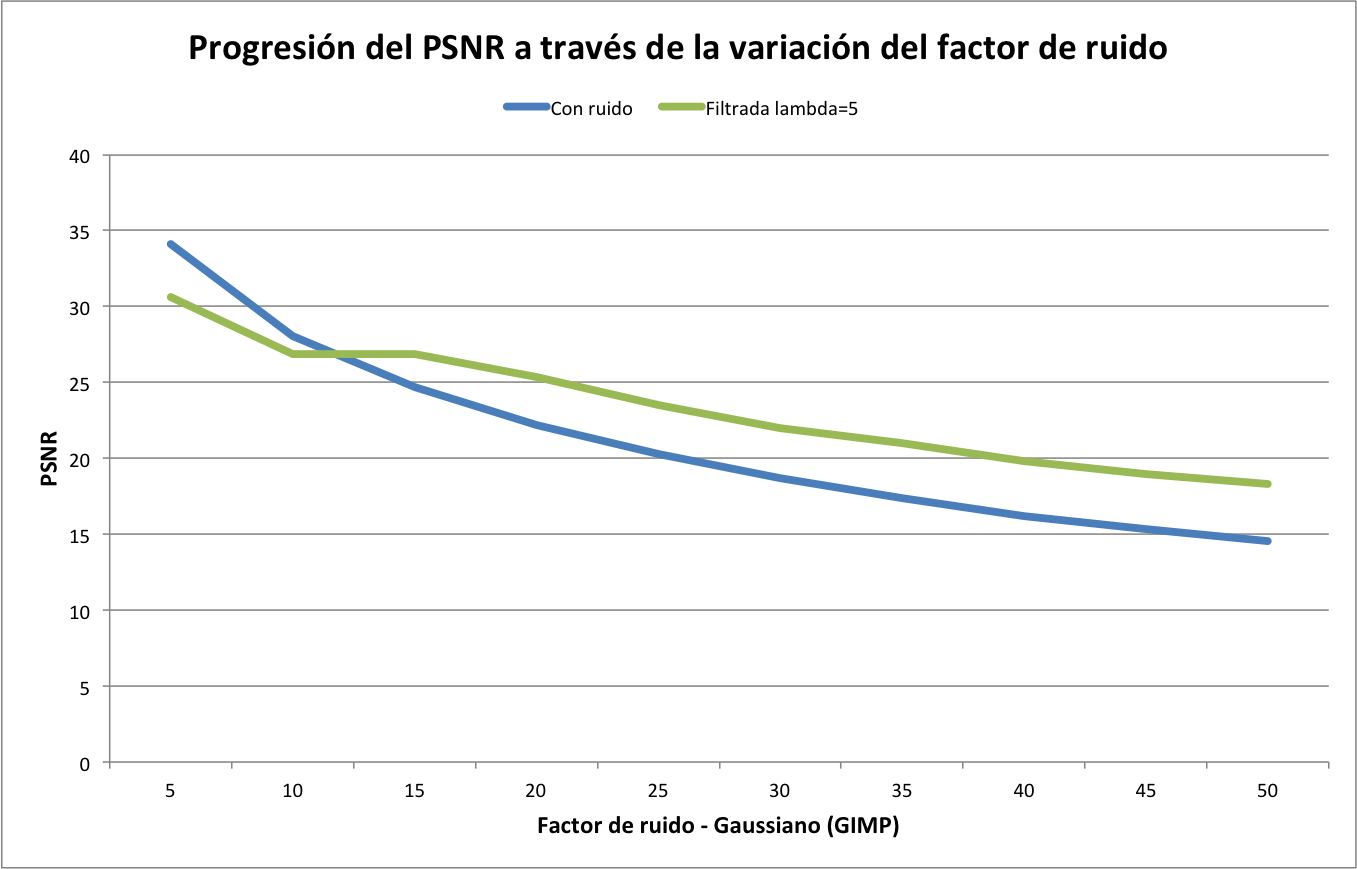
\includegraphics[scale=0.75]{graficos/PSNR_Einstein-GIMP.png}
  \caption{ Imágen de prueba: Einsten. Valores del PSNR cuando filtramos la imágen con ruido, variando el factor de ruido introducido con el GIMP.}
\end{figure}

En la \texttt{figura 1}  vemos la mejora que produce el filtro con respecto a la imágen con ruido para un $\lambda$ determinado. \\ 
El $\ \lambda = 5$, nos resulto muy conveniente para nuestro algoritmo dado que la mayoría de veces nos da una amplia mejora. 

Ahora que sabemos como se comporta con una imágen con ruido generado por una herramienta como el GIMP, nos enfocamos a comparar con nuestra propia implementación de inserción de ruido.
En la \texttt{figura 2} vamos a ver que tiene un comportamiento similar, y de hecho utilizamos otros $\lambda$ para mostrar que no es un caso particular. 
\begin{figure}[H]
  \centering
  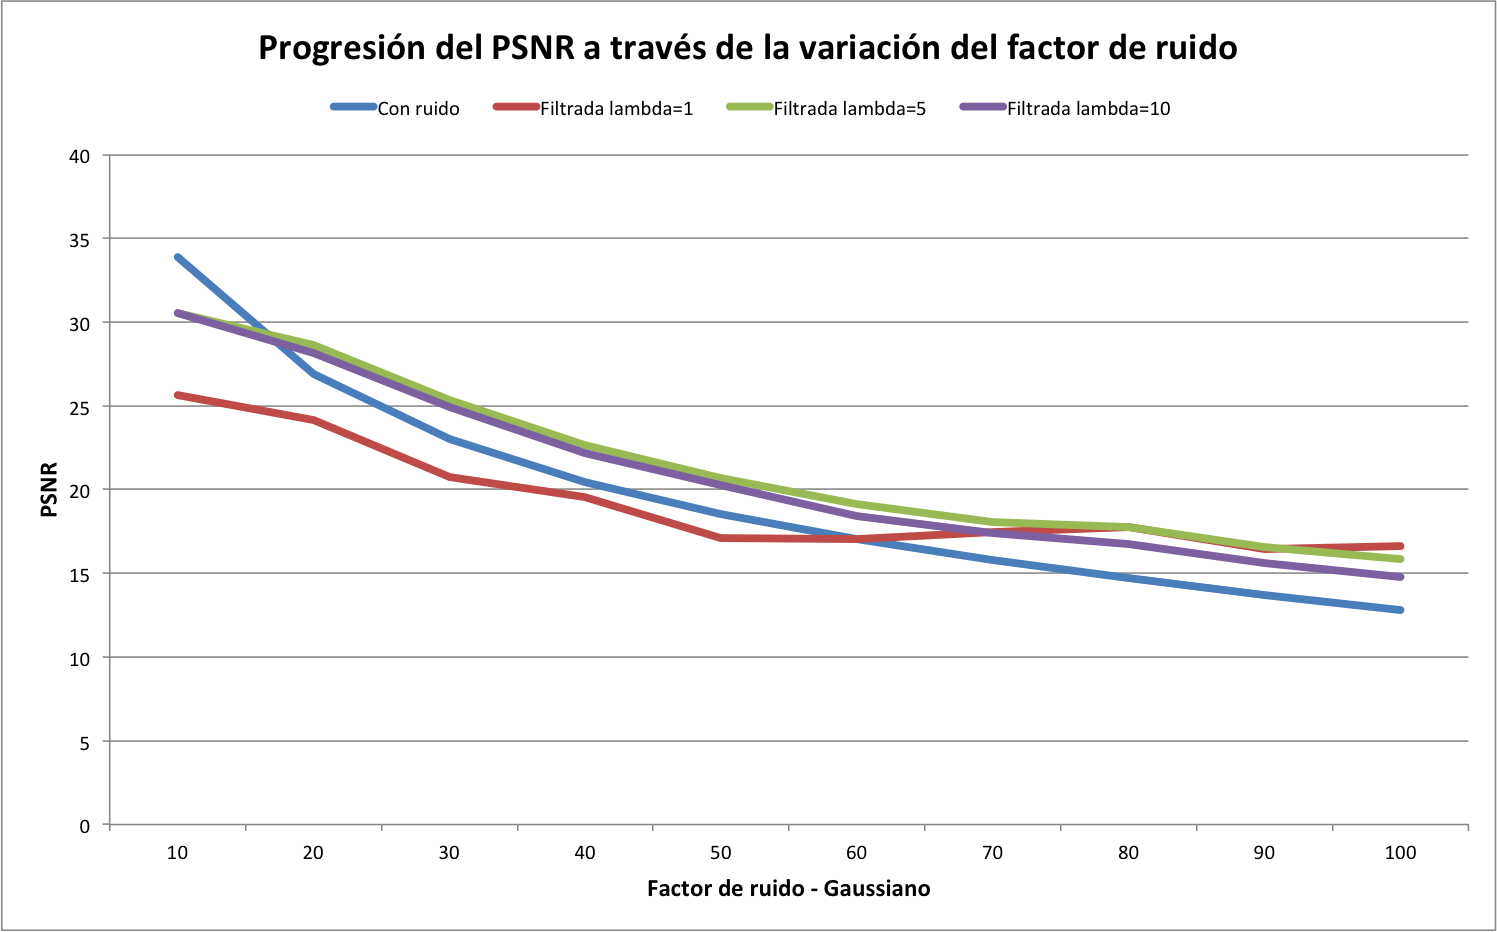
\includegraphics[scale=0.65]{graficos/PSNR_Einstein.png}
  \caption{ Imágen de prueba: Einsten. Valores del PSNR cuando filtramos la imágen con ruido introducido con nuestro algoritmo. }
\end{figure}

Mientras observamos el comportamiento partiendo de diferentes ruidos, notamos cierta relación entre el ruido y el $\lambda$.
Tomamos otra imágen y rehicimos todas las pruebas, y volcamos los resultados en el gráfico de la \texttt{figura 3}. 

\begin{figure}[H]
  \centering
  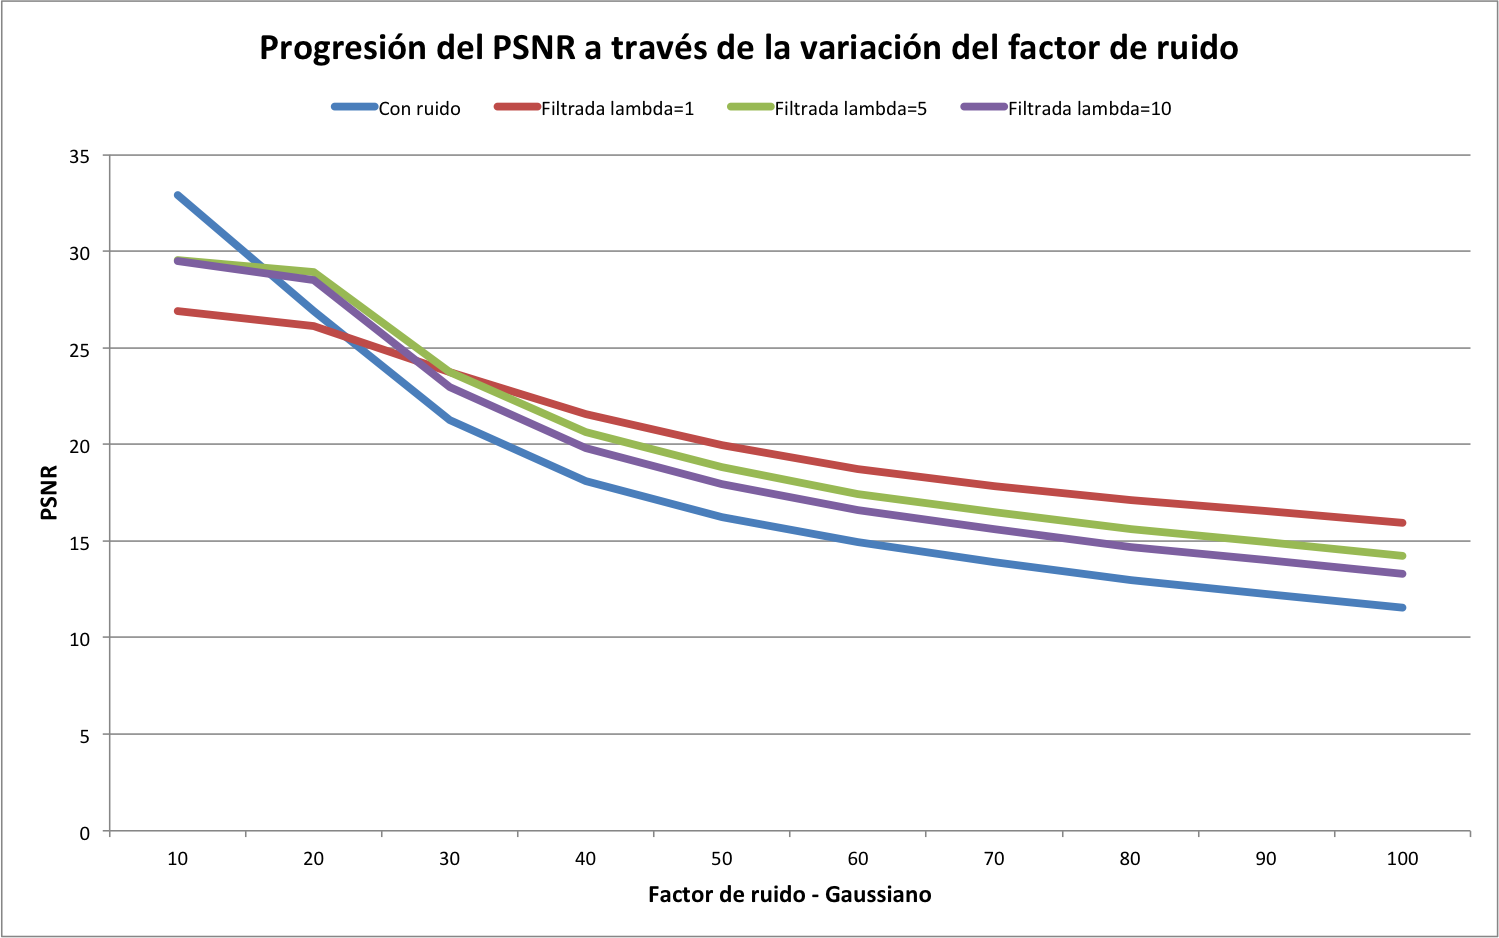
\includegraphics[scale=0.65]{graficos/PSNR_Blond.png}
  \caption{ Imágen de prueba: Blond. Valores del PSNR cuando filtramos la imágen con ruido, variando $\lambda$}
\end{figure}

Una vez más, encontramos la relación entre los parámetros. Para imágenes con poco ruido, nuestro filtro genera imágenes de mejor calidad con $\lambda$ más grandes. Y cuando el factor de \textit{ruido} es mayor, conviene seleccionar un $\lambda$ más chico.

Sin embargo, continuamos con las pruebas con otra imágen, y esta vez variando progresivamente el $\lambda$. Los resultados que obtuvimos fueron los siguientes: 

\vspace{2em}
\centering 
\begin{tabular}{|l|l|l|l|}
  \hline
  \multirow{2}{*}{$\lambda$} & \multicolumn{3}{|c|}{PSNR} \\
  \cline{2-4}
   & F.R. 10 & F.R. 50 & F.R. 100 \\ \hline

  Ruido	 & 	32.89	 & 	18.88	 & 	19.95 \\
  01	 & 	21.73	 & 	25.80	 & 	18.50 \\
  02	 & 	22.19	 & 	24.40	 & 	17.35 \\
  03	 & 	22.24	 & 	23.32	 & 	16.51 \\
  04	 & 	22.46	 & 	22.54	 & 	15.90 \\
  05	 & 	22.61	 & 	21.96	 & 	15.43 \\
  06	 & 	22.71	 & 	21.51	 & 	15.06 \\
  07	 & 	22.78	 & 	21.16	 & 	14.76 \\
  08	 & 	22.87	 & 	20.86	 & 	14.52 \\
  09	 & 	22.94	 & 	20.66	 & 	14.31 \\
  10	 & 	22.99	 & 	20.49	 & 	14.14 \\
  11	 & 	23.03	 & 	20.34	 & 	13.99 \\
  12	 & 	23.06	 & 	20.21	 & 	13.86 \\
  13	 & 	23.08	 & 	20.09	 & 	13.74 \\
  14	 & 	23.10	 & 	19.99	 & 	13.64 \\
  15	 & 	23.12	 & 	19.89	 & 	13.55 \\
  16	 & 	23.13	 & 	19.81	 & 	13.47 \\
  17	 & 	23.14	 & 	19.74	 & 	13.39 \\
  18	 & 	23.15	 & 	19.67	 & 	13.33 \\
  19	 & 	23.16	 & 	19.63	 & 	13.27 \\
  20	 & 	23.16	 & 	19.58	 & 	13.21 \\
  \hline
\end{tabular}

%Se incluira aquı un analisis de los resultados obtenidos en la seccion anterior (se analizara su validez, coherencia, etc.). Deben analizarse como mınimo los ıtems pedidos en el enunciado. No es aceptable decir que “los resultados fueron los esperados”, sin hacer clara referencia a la teor ́ıa a la cual se ajustan. Adem ́as, se deben mencionar los resul- tados interesantes y los casos “patol ́ogicos” encontrados.

\newpage

\section{Conclusiones}

%Esta secci ́on debe contener las conclusiones generales del trabajo. Se deben mencionar las relaciones de la discusi ́on sobre las que se tiene certeza, junto con comentarios y observaciones generales aplicables a todo el proceso. Mencionar tambi ́en posibles extensiones a los m ́etodos, experimentos que hayan quedado pendientes, etc.

\newpage

\section{Apéndices}

\subsection{A - Enunciado}

Un problema típico que se encuentra al trabajar con imágenes digitales es la existencia de ``ruido'' en las mismas. En pocas palabras, podemos decir que el ruido ocurre cuando el valor de uno o más píxeles de la imagen, no se corresponden con la realidad. La mayor\'ia de las veces, esto se debe a la calidad del equipo electr\'onico utilizado para tomar las fotograf\'ias, o bien a posibles perturbaciones introducidas al momento de transmitir la informaci\'on. Un caso muy com\'un de im\'agenes con ruido son las fotograf\'ias satelitales.

%Una forma de corregir (o reducir) este fen\'omeno en las im\'agenes es mediante la aplicaci\'on de filtros, con el objetivo de suavizar las mismas para obtener resultados m\'as cercanos a la realidad. Hoy en d\'ia, existen muchas t\'ecnicas de filtrado de im\'agenes,  muchas de ellas est\'an basadas en modelos matem\'aticos que en general se resuelven mediante m\'etodos num\'ericos.

Se puede pensar el problema de filtrar una imagen con ruido como la minimizaci\'on del siguiente funcional:
\begin{equation}
  \Pi = \int_\Omega {\frac{\lambda}{2} \left| u - \tilde{u} \right|^2 + \frac{1}{2} \lVert \nabla u \rVert^2 } d\Omega,
\label{funcional}
\end{equation}
donde $u : \Omega \subset \mathbb{R}^2 \to \mathbb{R}$ describe la imagen filtrada y
$\tilde{u} : \Omega \subset \mathbb{R}^2 \to \mathbb{R}$ la imagen a filtrar (con ruido).
De esta manera, el primer t\'ermino \emph{pesa} cuanto ruido tiene $\tilde{u}$ y el segundo \emph{pesa} la suavidad de la imagen obtenida. La constante $\lambda$ controla la importancia relativa de los dos t\'erminos.

La minimizaci\'on del funcional de la ecuaci\'on~(\ref{funcional}) da lugar a la siguiente ecuaci\'on diferencial:
% \begin{equation}
%  \lambda \left( u - \tilde{u} \right) - \nabla^2 u = 0.
% \label{ecdif}
% \end{equation}
\begin{equation}
 \lambda \left( u - \tilde{u} \right) - \left( \frac{\partial^2 u}{\partial x^2} + \frac{\partial^2 u}{\partial y^2} \right) = 0.
\label{ecdif}
\end{equation}

La soluci\'on de la ecuaci\'on~(\ref{ecdif}) que representa la imagen filtrada se puede aproximar de manera discreta utilizando el m\'etodo de diferencias finitas, lo cual conduce al siguiente sistema de ecuaciones:
\begin{equation}
 \lambda u_{i,j} - \left( u_{i-1,j} + u_{i+1,j} + u_{i,j-1} + u_{i,j+1} - 4 u_{i,j} \right) = \lambda \tilde{u_{i,j}}
 \label{eqlin}
\end{equation}
donde ahora $u,\tilde{u} : \Omega \subset \mathbb{Z}^2 \to [0 \dots 255]$ son la versiones discretas de la imagen filtrada y la imagen original, respectivamente. Viendo la imagen $u$ como una matriz, $i,j$ son los \'indices de fila y columna de cada elemento (p\'ixel)  de la matriz, donde el 0 es representado por el color negro y el 255 por el blanco\footnote{Este modelo de filtrado de im\'agenes se puede extender a im\'agenes color RGB, repitiendo el proceso descripto para cada componente de color.}.

{\bf Enunciado}

El objetivo principal de este trabajo pr\'actico es implementar un programa para eliminar (o reducir) el ruido en im\'agenes digitales. Para ello, el programa deber\'a tomar como entrada una imagen (supuestamente con ruido) y resolver la ecuaci\'on~(\ref{ecdif}) por el m\'etodo de diferencias finitas (resolviendo el sistema de ecuaciones dado por las ecuaciones~(\ref{eqlin})). Finalmente, el programa deber\'a devolver la versi\'on filtrada de la im\'agen. La constante $\lambda$ involucrada en las ecuaciones debe ser un par\'ametro del programa de manera tal que se pueda luego experimentar con ella.

Adicionalmente, el programa implementado deber\'a ser capaz de procesar im\'agenes de gran tama\~no. Para ello, se pide implementar una funcionalidad extra que permita reducir las im\'agenes antes de ser procesadas y que, luego del proceso, revierta esta reducci\'on para lograr as\'i una imagen de las dimensiones originales. El {\em factor de reducci\'on} a utilizar debe ser un par\'ametro del programa. Por ejemplo, si se desea procesar una imagen de 5 {\em megap\'ixeles}\footnote{Un megap\'ixel equivale a un mill\'on de p\'ixeles.}, puede ocurrir que el tiempo de proceso necesario exceda lo que uno est\'a dispuesto a esperar, con lo cual ser\'ia posible reducir la imagen con un cierto factor de reducci\'on y aplicar el proceso de filtrado a una imagen de menores dimensiones. Obviamente, la salida del programa deber\'a invertir este proceso para retornar una imagen de dimensiones id\'enticas a la imagen original. Estos procesos llevan el nombre de {\em submuestreo} (la reducci\'on) y {\em sobremuestreo} (la ampliaci\'on) y existen muchas formas de realizarlos. La manera de realizarlos para este trabajo queda a criterio del grupo.

% El proceso de filtrado descripto puede aplicarse tambi\'en en forma iterativa. Es decir, luego de la primer pasada de filtrado, es posible repetir el procedimiento sobre la imagen obtenida con el objetivo de seguir reduciendo el ruido en la misma. El programa implementado deber\'a permitir realizar este proceso iterativo y la cantidad de iteraciones deber\'a ser un par\'ametro del programa, sobre el cual sea posible experimentar.

Tanto el valor de la constante $\lambda$ como el factor de reducci\'on
%  y la cantidad de iteraciones de filtrado 
tendr\'an un fuerte impacto en la calidad de las im\'agenes obtenidas. 
% Los dos \'ultimos impactar\'an 
El factor de reducci\'on impactar\'a
tambi\'en en los tiempos de ejecuci\'on. Para medir estos impactos, se deber\'a realizar una experimentaci\'on computacional cuyos resultados deber\'an ser plasmados en el informe del trabajo.

{\bf Experimentaci\'on}

Una forma de medir la calidad visual de las im\'agenes filtradas, es a trav\'es del PSNR ({\em Peak Signal-to-Noise Ratio}).
EL PSNR es una m\'etrica ``perceptual'' (acorde a lo que perciben los humanos) y nos da una forma de medir la calidad de una imagen perturbada, siempre y cuando se cuente con la imagen original. 
Cuanto mayor es el PSNR mayor es la calidad de la imagen. La unidad de medida es el decibel (db) y se considera que una diferencia de 0.5 db ya es notada por la vista humana. El PSNR se define como:
$$
\mathit{PSNR} = 10 \cdot \log_{10} \left( \frac{\mathit{MAX}^2_u}{\mathit{ECM}} \right)
$$
donde $MAX_u$ define el rango m\'aximo de la imagen (para nuestro caso ser\'ia 255) y ECM es el {\em error cuadr\'atico medio}, definido como:
$$
\frac{1}{N} \sum_{i,j}{(u^0_{i,j} - u_{i,j})^2} 
$$
donde $N$ es la cantidad de p\'ixeles de la imagen, $u^0$ es la imagen original y $u$ es la imagen perturbada (o en nuestro caso, la imagen recuperada).

La experimentaci\'on propuesta para el presente trabajo pr\'actico consiste en analizar la calidad de las im\'agenes reconstru\'idas y los tiempos de ejecuci\'on en funci\'on de: \\[-8mm]
	\begin{itemize}
		\item el nivel de ruido en la imagen, \\[-6mm]
		\item la constante $\lambda$ y\\[-6mm]
		\item el factor de reducci\'on. \\[-6mm]
% 		\item la cantidad de iteraciones de filtrado. \\[-8mm]
	\end{itemize}	
	
Dado que para medir la calidad se requiere contar con la imagen original, se deber\'an utilizar im\'agenes \emph{ruidosas} generadas artificialmente (por ejemplo, sumando o restando a los p\'ixeles de la imagen original valores generados aleatoriamente con distribuci\'on uniforme).
	
{\bf Formatos de archivos de entrada}

Para leer y escribir im\'agenes sugerimos utilizar el formato {\em raw} binario \texttt{.pgm}\footnote{\url{http://netpbm.sourceforge.net/doc/pgm.html}}. 
El mismo es muy sencillo de implementar y compatible con muchos gestores de fotos\footnote{XnView \url{http://www.xnview.com/}} y Matlab.

\newpage

\subsection{B - Cómo compilar y usar el TP}
El directorio del TP contiene un Makefile, con lo cual para compilarlo basta sólamente con ejecutar \textbf{make}. Los binarios generados son: 

\begin{itemize}
  \item \textbf{tp} Lee la imagen, plantea el sistema de equaciones, aplica el algoritmo de Gauss y resuelve el sistema. Luego graba la nueva imagen
  \begin{description}
	\item[-l] Lambda.
	\item[-f] Ruta de la foto con ruido.
	\item[-o] Ruta de la foto filtrada.
	\item[-r] Factor de reducción [Entero].
  \end{description}


  \item \textbf{psnr} Calcula el PSNR de las fotos pasadas como parámetro.
  \begin{description}
	\item[-c] Ruta de la foto sin ruido.
	\item[-n] Ruta de la foto con ruido.
  \end{description}

  \item \textbf{generateNoise} Agrega ruido a la foto
  \begin{description}
	\item[-M] es el método a ejecutar y se mapean del siguiente modo:
	\begin{itemize}
	   \item 0 para Salt \& Pepper
	   \item 1 para Gaussian
         \end{itemize}

	\item[-f] Ruta de la foto a agregar ruido.
	\item[-o] Ruta de la foto con ruido.
	\item[-p] Parámetro P para \textbf{Salt \& Pepper}
	\item[-q] Parámetro Q para \textbf{Salt \& Pepper}
	\item[-r] Factor para \textbf{Gaussian}
  \end{description}

\end{itemize}

\newpage

%\section{Referencias TODO}
%Es importante incluir referencias a libros, art ́ıculos y p ́aginas de Internet consultados durante el desarrollo del trabajo, haciendo referencia a estos materiales a lo largo del informe. Se deben citar tambi ́en las comunicaciones personales con otros grupos.


\end{document}
